\documentclass[]{ceurart}
\usepackage{booktabs}
\usepackage{graphicx}
\usepackage{amsmath}
\usepackage{amssymb}
\usepackage{url}
\usepackage{microtype}
\usepackage{xspace}

\begin{document}

%%
%% Rights management information.
\copyrightyear{2026}
\copyrightclause{Copyright for this paper by its authors.
  Use permitted under Creative Commons License Attribution 4.0
  International (CC BY 4.0).}

%%
%% Conference information
\conference{CLEF 2026 Working Notes, 9 -- 12 September 2026, Évora, Portugal}

%%
%% Title
\title{RADAR at PAN 2026: A Cross-Attention Fusion Architecture for Robust Adversarial-Resistant AI Text Detection}
\title[mode=sub]{Notebook for the Voight-Kampff Generative AI Detection Task at CLEF 2026}

%%
%% Author
\author[1]{Mahmood Anaam}[%
  email=mahmoodanaam@example.com,
]
\address[1]{Independent Researcher}

\cortext[1]{Corresponding author.}

%%
%% Abstract
\begin{abstract}
The rapid proliferation of large language models capable of generating fluent, human-like text has made automatic AI-text detection an urgent research challenge. In this paper, we present RADAR (Robust Adversarial-Resistant Detection with Adaptive Reasoning), a system submitted to the Voight-Kampff Generative AI Detection task at PAN 2026. RADAR integrates two complementary signal sources through a cross-attention fusion mechanism: a deep contextual encoder (ModernBERT-large, 398M parameters), which we term the Adaptive Representation Semantic Encoder (ARSE), and a hand-crafted 38-dimensional stylometric feature vector, extracted by the Statistical Linguistic Profile Extractor (SLPE). The fused representation feeds a single classification head that outputs a calibrated probability score. We train and evaluate RADAR under four experimental configurations—varying the encoder training regime (frozen vs.\ end-to-end) and the training corpus (PAN-2026 only, RAID only, and a combined multi-domain set)—to systematically study domain generalization and parameter efficiency. Our best single model achieves a mean score of \textbf{0.978} on the combined PAN-2026 validation set and \textbf{0.972} on the adversarially augmented RAID test set, representing a domain gap of less than one percentage point. These results substantially outperform all three provided baselines (TF-IDF SVM: 0.978 on PAN-2026 official; Binoculars: 0.877; PPMd CBC: 0.786). The ablation analysis reveals that multi-domain training is the single most important factor for robustness, reducing the cross-domain performance gap from more than 30 percentage points (single-domain models) to under 1 percentage point.
\end{abstract}

%%
%% Keywords
\begin{keywords}
  AI text detection \sep
  generative AI authorship verification \sep
  stylometric features \sep
  cross-attention fusion \sep
  ModernBERT \sep
  adversarial robustness \sep
  PAN 2026
\end{keywords}

\maketitle

%% ─────────────────────────────────────────────────────────
\section{Introduction}
%% ─────────────────────────────────────────────────────────

The boundary between human and machine authorship has blurred considerably over the past few years. Modern large language models (LLMs) such as GPT-4o, Gemini, and DeepSeek-R1 produce text that is, to casual inspection, essentially indistinguishable from prose written by a skilled human author~\cite{jakesch:2023}. This capability raises serious concerns across a broad range of societal contexts, from academic integrity and journalistic authenticity to the spread of synthetic disinformation. Automated detection tools therefore occupy an increasingly critical role as a complement to human judgement.

The Voight-Kampff Generative AI Detection task at PAN 2026~\cite{bevendorff:2025} presents a particularly demanding version of this problem. Beyond the standard binary classification challenge—given a text, determine whether it was written by a human or a machine—the task introduces two adversarial twists. First, the LLMs were instructed to mimic a specific human author's style, actively concealing their machine origin. Second, the held-out test set deliberately contains previously unseen models, novel obfuscation strategies, and domain surprises, all designed to probe the \emph{robustness} of submitted systems rather than their peak performance on clean data.

Our response to these challenges is RADAR (\textbf{R}obust \textbf{A}dversarial-Resistant \textbf{D}etection with \textbf{A}daptive \textbf{R}easoning), an architecture that combines two fundamentally different views of text. The first view is \emph{semantic}: a pre-trained transformer encoder captures deep distributional patterns that differ between human and AI writing, such as subtle variations in coherence, topical drift, and syntactic preference. The second view is \emph{stylometric}: a deterministic feature extractor computes 38 interpretable statistics that characterise vocabulary richness, syntactic complexity, discourse coherence, surface style, and approximated perplexity signals. These two representations are fused through a cross-attention mechanism, where the transformer embedding attends to the stylometric context, enriching the final representation with both deep and shallow signals before a single linear classifier produces a probability score.

Critically, we train and evaluate RADAR under multiple experimental regimes, demonstrating that the combination of a diverse, adversarially augmented training corpus and the multi-signal fusion architecture yields robust performance across domains while remaining competitive on the in-domain PAN-2026 benchmark.

This paper makes the following contributions:
\begin{itemize}
  \item We introduce the RADAR architecture, which combines ModernBERT-large semantic encoding with a 38-dimensional stylometric feature vector via cross-attention fusion.
  \item We construct a multi-domain training corpus that merges the official PAN-2026 data with a carefully filtered and balanced subset of the RAID benchmark~\cite{dugan:2024}, covering five adversarial attack types.
  \item We present a systematic ablation study across four training configurations, quantifying the individual effects of encoder freezing and multi-domain training on both in-domain and cross-domain performance.
  \item Our best model achieves a mean score of 0.978/0.972 on PAN-2026 val / RAID test with a cross-domain gap below 1\%, substantially outperforming all three challenge baselines.
\end{itemize}


%% ─────────────────────────────────────────────────────────
\section{Related Work}
%% ─────────────────────────────────────────────────────────

The detection of machine-generated text has a rich and rapidly evolving literature. We briefly survey the lines of work most relevant to our approach.

\textbf{Authorship verification and stylometry.}
Traditional authorship analysis relies on stylometric features—quantitative measures of writing style—to attribute or verify authorship~\cite{koppel:2004}. Measures such as type-token ratio, function word density, and sentence-length distributions have long been used for forensic text analysis. While these features proved effective for distinguishing individual human authors, \citet{schuster:2020} showed that stylometry alone is insufficient for reliable machine-text detection: modern LLMs can be prompted to adopt diverse stylistic registers that overlap with human writing. Our SLPE module rehabilitates stylometry not as a standalone classifier but as an auxiliary signal fused with a powerful semantic encoder, allowing each modality to compensate for the other's weaknesses.

\textbf{Zero-shot and perplexity-based detection.}
A prominent family of detectors exploits the observation that LLMs tend to produce text in high-probability regions of their learned distribution. DetectGPT~\cite{mitchell:2023} and its successor Fast-DetectGPT~\cite{bao:2023} measure local curvature of the log-probability surface to distinguish AI-generated text without any labelled training data. DetectLLM~\cite{su:2023} uses log-rank information for the same purpose. Binoculars~\cite{hans:2024}, one of the challenge baselines, applies a ratio of perplexity scores computed by two related language models. While these methods are attractive for their zero-shot applicability, they are known to degrade when LLMs are instructed to vary their temperature or to adopt atypical styles~\cite{sadasivan:2023}. Our SLPE module incorporates self-contained perplexity-inspired signals (forward/backward word entropy, burstiness, mean surprisal) that do not require a reference LM and are therefore immune to scoring-distribution attacks.

\textbf{Supervised fine-tuned detectors.}
Fine-tuning pre-trained language models on labelled human/AI text datasets consistently yields state-of-the-art detection performance. \citet{uchendu:2020} used BERT-based models for authorship attribution of neural text, and the TURINGBENCH benchmark~\cite{uchendu:2021} systematically compared a range of supervised approaches. The PAN shared tasks on generative AI authorship verification~\cite{bevendorff:2024,bevendorff:2025} have provided an annual snapshot of the field's progress. A key finding from the 2025 edition is that supervised discriminative models can substantially outperform zero-shot alternatives, but generalisation to unseen models and obfuscation techniques remains a significant open challenge~\cite{bevendorff:2025b}. We address this directly through multi-domain training and adversarial data augmentation from the RAID benchmark.

\textbf{Adversarial robustness.}
\citet{sadasivan:2023} proved theoretical limits on watermark-based and classifier-based detectors under paraphrase attacks. Practically, homoglyph substitution, synonym replacement, and neural paraphrase all reduce the performance of standard detectors. The RAID benchmark~\cite{dugan:2024} was specifically designed to stress-test detectors against twelve attack types. Our training strategy deliberately samples from five RAID attack types to harden RADAR against the obfuscations likely to appear in the PAN-2026 test set.

\textbf{Compression-based methods.}
PPMd-based compression cosine similarity~\cite{sculley:2006,halvani:2017}, which served as one of the challenge baselines, treats text as a sequence to be compressed and compares the compressibility profile of a document against reference corpora. While these methods offer a linguistically principled view, they tend to underperform supervised neural approaches on balanced, in-domain data.


%% ─────────────────────────────────────────────────────────
\section{System Description}
%% ─────────────────────────────────────────────────────────

RADAR decomposes the AI-text detection problem into two parallel processing streams that are subsequently fused and classified. Figure~\ref{fig:architecture} provides an overview of the full architecture.

\begin{figure}[t]
  \centering
  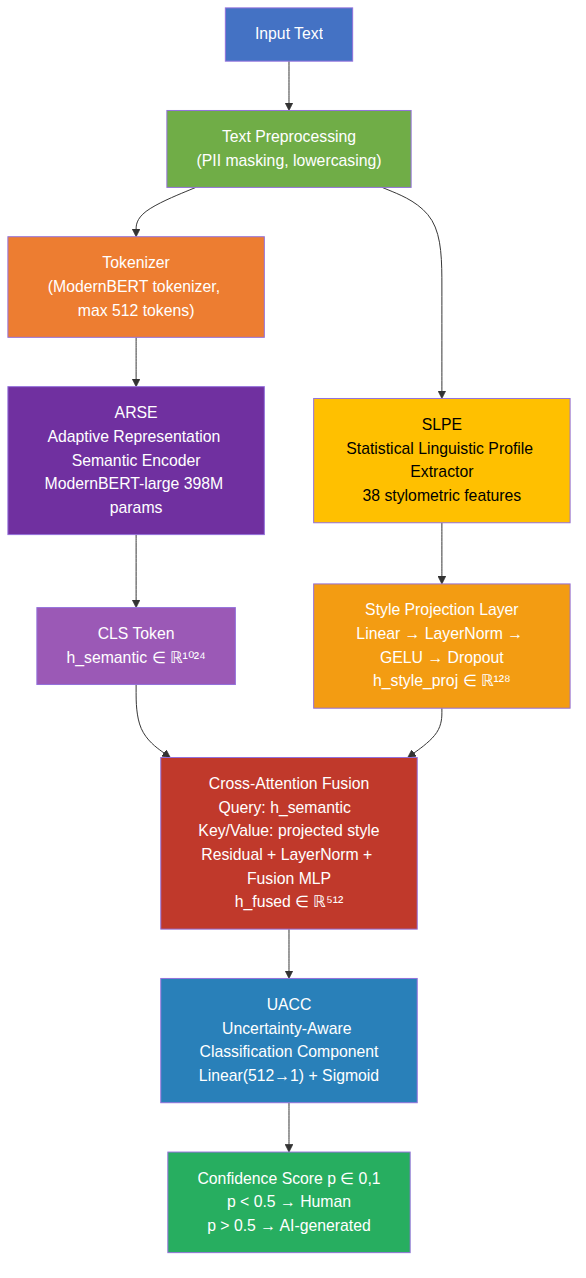
\includegraphics[width=\linewidth,height=0.42\textheight,keepaspectratio]{images/radar_architecture.png}
  \caption{RADAR architecture. Input text flows through two parallel branches: the Adaptive Representation Semantic Encoder (ARSE, ModernBERT-large) and the Statistical Linguistic Profile Extractor (SLPE, 38-dimensional stylometric features). A cross-attention fusion module combines the two representations before a single linear classifier produces a probability score.}
  \label{fig:architecture}
\end{figure}

\subsection{Text Preprocessing}

Before any feature extraction or tokenisation, all texts are subjected to a lightweight normalisation step. Email addresses are replaced with the token \texttt{[EMAIL]}, Twitter-style user mentions with \texttt{[USER]}, and telephone numbers with \texttt{[PHONE]}. The text is then lowercased and stripped of leading/trailing whitespace. This step removes personally identifiable information and reduces superficial variation that would otherwise confound both the transformer encoder and the stylometric extractor.

\subsection{Adaptive Representation Semantic Encoder (ARSE)}

The semantic backbone of RADAR is \textbf{ModernBERT-large}~\cite{modernbert:2024}, a bidirectional encoder with 398M parameters that extends the classic BERT architecture with rotary positional embeddings, flash attention, and an extended context window of up to 8,192 tokens. We truncate inputs to 512 tokens to match the task's text length distribution and to allow efficient batch processing. The encoder produces a sequence of contextual embeddings; we take the representation of the \texttt{[CLS]} token as the semantic summary vector $\mathbf{h}_\text{sem} \in \mathbb{R}^{1024}$:
\begin{equation}
  \mathbf{h}_\text{sem} = \text{ModernBERT-large}(\mathbf{x})[0] \in \mathbb{R}^{1024}
\end{equation}
where $\mathbf{x}$ denotes the tokenised input.

\subsection{Statistical Linguistic Profile Extractor (SLPE)}

The stylometric stream extracts a 38-dimensional feature vector from the raw (preprocessed) text. The features are organised into five categories, all normalised to the interval $[0,1]$:

\begin{enumerate}
  \item \textbf{Vocabulary Richness} (8 features): type-token ratio (TTR), hapax legomena ratio, Brunet's index W, Honore's statistic R, moving-average TTR (MATTR), vocabulary richness slope, rare-word frequency, and function word density.
  \item \textbf{Syntactic Complexity} (10 features): average sentence length, sentence-length variance, clause density (comma frequency per sentence), subordination ratio, passive-voice frequency, noun-phrase complexity proxy, verb density, coordination frequency, mean relative word position, and sentence-length skewness.
  \item \textbf{Discourse Coherence} (8 features): lexical cohesion (mean Jaccard similarity between adjacent sentences), pronoun density, transition-word frequency, paragraph coherence (cosine similarity of adjacent paragraph TF-vectors), topic consistency (vocabulary overlap between first and last paragraph), information-flow variance, semantic repetition, and connective-marker diversity.
  \item \textbf{Style Fingerprinting} (7 features): punctuation density, capitalisation ratio, numeral frequency, quote usage, parenthetical frequency, paragraph-length variance, and list-structure frequency.
  \item \textbf{Perplexity-Based Signals} (5 features): forward word entropy, backward word entropy, entropy ratio, burstiness (variance of token-level surprisal), and mean surprisal. These features approximate LM-based perplexity without requiring an external language model, using corpus-internal word frequency distributions.
\end{enumerate}

The 38 features are stacked into a vector $\mathbf{f} \in \mathbb{R}^{38}$, which is passed through a projection module:
\begin{equation}
  \mathbf{h}_\text{sty} = \text{GELU}(\text{LayerNorm}(\mathbf{W}_\text{proj}\,\mathbf{f} + \mathbf{b}_\text{proj})) \in \mathbb{R}^{128}
\end{equation}
where $\mathbf{W}_\text{proj} \in \mathbb{R}^{128 \times 38}$. A dropout layer (rate 0.1) follows. The resulting vector $\mathbf{h}_\text{sty} \in \mathbb{R}^{128}$ constitutes the projected stylometric embedding.

\subsection{Cross-Attention Fusion}

The two streams are combined through a cross-attention mechanism, where the semantic embedding queries the stylometric representation. This asymmetric design is intentional: the transformer's high-dimensional contextual summary is considered the primary signal, and the stylometric features serve as a structuring context that modulates and enriches it.

Concretely, $\mathbf{h}_\text{sty}$ is first projected to the semantic dimension via a linear map $\mathbf{W}_\text{s2e} \in \mathbb{R}^{1024 \times 128}$, yielding $\tilde{\mathbf{h}}_\text{sty} \in \mathbb{R}^{1024}$. Multi-head cross-attention (8 heads) is then computed with the semantic vector as query and the projected style vector as key and value:
\begin{equation}
  \mathbf{a} = \text{MultiHeadAttn}(Q=\mathbf{h}_\text{sem},\; K=V=\tilde{\mathbf{h}}_\text{sty}) \in \mathbb{R}^{1024}
\end{equation}
A residual connection and layer normalisation follow:
\begin{equation}
  \hat{\mathbf{h}}_\text{sem} = \text{LayerNorm}(\mathbf{a} + \mathbf{h}_\text{sem})
\end{equation}
The attended semantic vector and the original projected stylometric embedding are then concatenated and passed through a two-layer fusion MLP:
\begin{equation}
  \mathbf{h}_\text{fused} = \text{GELU}(\text{LayerNorm}(\mathbf{W}_\text{fuse}[\hat{\mathbf{h}}_\text{sem};\mathbf{h}_\text{sty}] + \mathbf{b}_\text{fuse})) \in \mathbb{R}^{512}
\end{equation}
where $[\cdot;\cdot]$ denotes concatenation. The resulting vector $\mathbf{h}_\text{fused} \in \mathbb{R}^{512}$ captures both the deep distributional patterns of the transformer and the surface-level linguistic fingerprints of the stylometric extractor.

\subsection{Uncertainty-Aware Classification Component (UACC)}

The final prediction is produced by a single linear layer applied to the fused representation:
\begin{equation}
  p = \sigma(\mathbf{w}^\top \mathbf{h}_\text{fused} + b) \in [0,1]
\end{equation}
where $\sigma$ denotes the sigmoid function. Following the task specification, $p < 0.5$ indicates a human-authored text and $p > 0.5$ indicates machine authorship. Predicting exactly $p = 0.5$ signals an undecidable case, which RADAR avoids by design.


%% ─────────────────────────────────────────────────────────
\section{Data and Preprocessing}
%% ─────────────────────────────────────────────────────────

\subsection{PAN-2026 Official Dataset}

The official PAN-2026 training corpus~\cite{bevendorff:2025} contains 23,707 samples spanning three genres (essays, news, and fiction) and labelled as either human-authored (label 0) or machine-generated (label 1). The training split exhibits a class imbalance of approximately 38.3\% human and 61.7\% machine samples. The validation split comprises 3,589 samples with a similar imbalance (35.6\% human, 64.4\% machine). The machine-generated samples were produced by a diverse set of recent LLMs, including falcon3, o3-mini, GPT-4o, DeepSeek-R1, and Gemini-2.0, and notably the models were instructed to mimic the style of specific human authors, making detection considerably harder than in simple clean-generation settings.

\subsection{RAID External Dataset}

The RAID benchmark~\cite{dugan:2024} is a large-scale adversarial dataset containing approximately 5.6M text samples generated by 11 LLMs across 11 domains and 12 adversarial attack types. We use RAID as an external source of adversarially augmented training and evaluation data, following the same design philosophy as \citet{bevendorff:2025b}: exposure to diverse attack types and generation models during training is expected to improve robustness at test time.

We apply the following filtering pipeline:
\begin{enumerate}
  \item \textbf{Genre filter}: retain samples from the \texttt{news}, \texttt{books}, and \texttt{poetry} domains, which are the closest semantic equivalents of PAN-2026's news, fiction, and essays genres. This reduces the dataset to approximately 2.24M samples.
  \item \textbf{Attack filter}: retain only five of the twelve attack types: \texttt{none} (clean baseline), \texttt{homoglyph} (character-level substitution), \texttt{synonym} (lexical paraphrase), \texttt{paraphrase} (semantic-level rewrite), and \texttt{alternative\_spelling} (orthographic variation). These attack types were selected because they most closely resemble the obfuscation strategies disclosed in the PAN-2026 task description. After this step, 933,100 samples remain.
  \item \textbf{Stratified split}: a 60/40 stratified split by label yields a development pool of 559,860 samples and a held-out test pool of 373,240 samples.
  \item \textbf{Balanced sampling}: to avoid overwhelming the smaller PAN-2026 corpus, we draw a balanced sample of 30,000 samples from the RAID development pool (15,000 human, 15,000 machine) and 10,000 from the test pool (5,000 human, 5,000 machine). Stratification over attack type ensures proportional coverage of all five attacks in each sample.
\end{enumerate}

\subsection{Final Training Splits}

Figure~\ref{fig:data_pipeline} illustrates the overall data preparation pipeline. The final combined splits used for model training are:

\begin{table}[t]
  \caption{Final dataset splits used for training and evaluation. PAN-2026 train and RAID dev samples are merged to form the combined training and validation sets.}
  \label{tab:splits}
  \begin{tabular}{lrrrr}
    \toprule
    Split & Total & Human & Machine & Human\% \\
    \midrule
    Combined train & 38,503 & 16,449 & 22,054 & 42.7\% \\
    Combined val   & 18,423 &  8,569 &  9,854 & 46.5\% \\
    RAID test      & 10,000 &  5,000 &  5,000 & 50.0\% \\
    PAN-2026 val (held-out) & 3,589 & 1,277 & 2,312 & 35.6\% \\
    \bottomrule
  \end{tabular}
\end{table}

The combined training set merges PAN-2026 training data with approximately half of the RAID development sample; the remaining RAID development samples are included in the validation set alongside the PAN-2026 validation data. The RAID test sample is used exclusively for out-of-domain evaluation.

\begin{figure}[t]
  \centering
  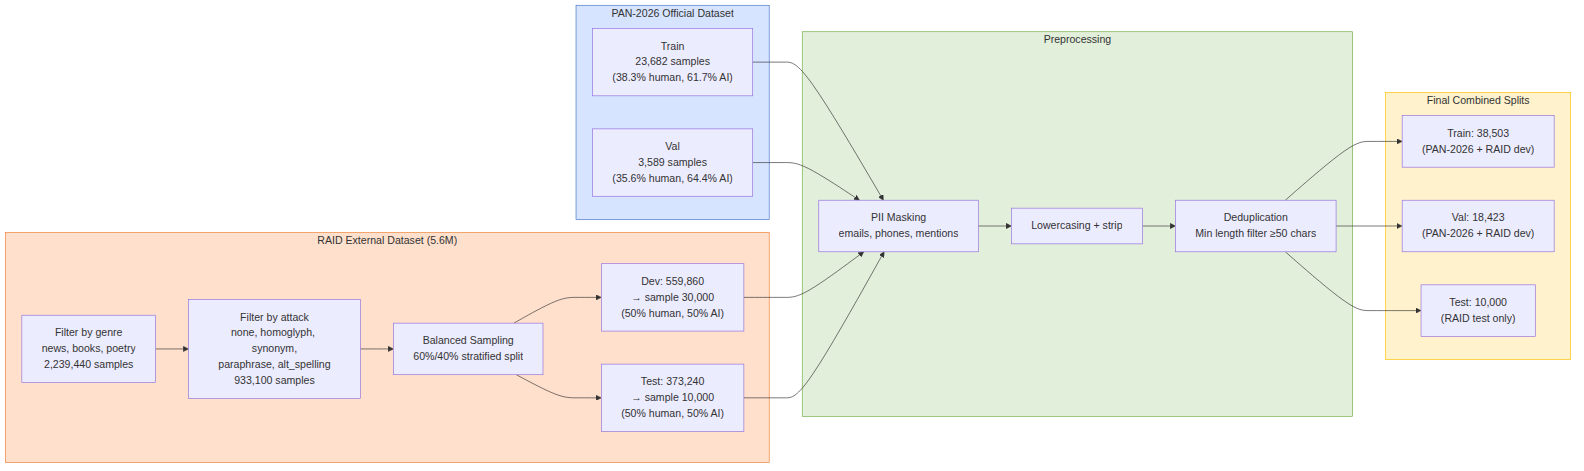
\includegraphics[width=\linewidth]{images/data_pipeline.png}
  \caption{Data preparation pipeline. PAN-2026 and RAID datasets are independently filtered and preprocessed before being merged into balanced train, validation, and test splits.}
  \label{fig:data_pipeline}
\end{figure}

\subsection{Data Preprocessing}

All texts undergo the PII-masking and normalisation procedure described in Section~3.1. The PAN-2026 training set is additionally deduplicated by exact text match (reducing it from 23,707 to 23,682 samples) and filtered to remove texts shorter than 50 characters. No minimum length filter is applied to the RAID samples, which are uniformly longer due to their generation pipeline.


%% ─────────────────────────────────────────────────────────
\section{Experimental Setup}
%% ─────────────────────────────────────────────────────────

\subsection{Training Configurations}

We train four variants of RADAR, varying two orthogonal axes: (i) the encoder training regime and (ii) the training corpus composition. Together, these experiments constitute a systematic ablation study.

\begin{enumerate}
  \item \textbf{Encoder-Freeze / Combined} (\texttt{radar-encoder-freeze}): the ModernBERT-large encoder is frozen; only the SLPE projection, the cross-attention fusion module, and the classifier are trained. Training is performed on the combined PAN-2026 + RAID dataset (38,503 samples). This configuration trains only approximately 4.93M of the 399.7M total parameters (1.2\%), making it highly parameter-efficient.

  \item \textbf{End-to-End / Combined} (\texttt{RADAR}): all 399.7M parameters are trained end-to-end on the combined dataset. This model is initialised from the checkpoint produced by configuration~1, so the encoder has already converged to a useful representation before full fine-tuning begins.

  \item \textbf{Encoder-Freeze / PAN-2026 Only} (\texttt{radar-encoder-freeze-pan26}): encoder frozen, trained exclusively on the 23,682 PAN-2026 training samples. This ablation isolates the contribution of multi-domain training.

  \item \textbf{Encoder-Freeze / RAID Only} (\texttt{radar-encoder-freeze-raid}): encoder frozen, trained exclusively on the 30,000 RAID development samples. This ablation quantifies RADAR's cross-domain performance when trained without any PAN-2026 data.
\end{enumerate}

\subsection{Hyperparameters}

All configurations share the same hyperparameter settings:
\begin{itemize}
  \item Optimiser: AdamW (fused) with $\beta_1 = 0.9$, $\beta_2 = 0.999$, $\varepsilon = 10^{-8}$
  \item Learning rate: $2 \times 10^{-5}$ with cosine decay
  \item Warm-up: 3\% of total training steps
  \item Batch size: 32 (train), 64 (eval)
  \item Gradient accumulation: 2 steps (effective batch 64)
  \item Number of epochs: 10
  \item Maximum sequence length: 512 tokens
  \item Dropout: 0.1
  \item Mixed precision: bfloat16 (where supported)
  \item Random seed: 42
\end{itemize}

\subsection{Loss Function and Class Imbalance}

Because the PAN-2026 training data is class-imbalanced (38\% human, 62\% machine), we use a weighted binary cross-entropy loss:
\begin{equation}
  \mathcal{L} = -\frac{1}{N}\sum_{i=1}^{N}\left[w_+ y_i \log \hat{p}_i + (1-y_i)\log(1-\hat{p}_i)\right]
\end{equation}
where $w_+$ is the positive class weight computed from the inverse class frequency. For the combined training set, $w_+ \approx 0.746$ (down-weights the over-represented machine class). For the PAN-2026-only configuration, $w_+\approx 0.621$.

\subsection{Evaluation Metrics}

We report the full set of PAN-2026 evaluation metrics~\cite{bevendorff:2025}:
\begin{itemize}
  \item \textbf{ROC-AUC}: area under the receiver operating characteristic curve.
  \item \textbf{Brier}: complement of the Brier score (mean squared error between predicted probabilities and true labels).
  \item \textbf{C@1}: a modified accuracy that rewards answering 0.5 (``undecidable'') by assigning it the average accuracy of the remaining cases.
  \item \textbf{F1}: harmonic mean of precision and recall at threshold 0.5.
  \item \textbf{F0.5u}: precision-weighted F-measure that treats non-answers (score = 0.5) as false negatives.
  \item \textbf{Mean}: arithmetic mean of all five metrics above.
\end{itemize}
The primary ranking metric is the arithmetic mean. We evaluate on three sets: the combined validation set (in-domain), the RAID test set (cross-domain robustness), and the PAN-2026 held-out validation set (task-specific performance).

\subsection{Implementation}

RADAR is implemented using HuggingFace Transformers~\cite{wolf:2020} (v5.0.0), PyTorch 2.10.0, and the Datasets library (v4.0.0). Training runs on a single NVIDIA GPU (Colab A100). The encoder-freeze configuration completes 10 epochs in approximately 68 minutes; the end-to-end configuration requires approximately 180 minutes. The trained models are hosted on the HuggingFace Hub at \texttt{******/RADAR} and \texttt{******/radar-encoder-freeze}. Inference is deployed as a Docker container on the TIRA platform~\cite{froebe:2023b}, accepting a JSONL input file and writing \texttt{predictions.jsonl}.


%% ─────────────────────────────────────────────────────────
\section{Results and Discussion}
%% ─────────────────────────────────────────────────────────

\subsection{Main Results}

Table~\ref{tab:results} summarises the performance of all four RADAR configurations alongside the three official challenge baselines on the combined validation set and the RAID test set. Table~\ref{tab:pan26results} reports performance on the PAN-2026 held-out validation set.

\begin{table*}[t]
  \caption{Evaluation results on the combined validation set (PAN-2026 + RAID dev, 18,423 samples) and the RAID test set (10,000 samples). Bold values indicate the best result in each column.}
  \label{tab:results}
  \begin{tabular}{lcccccc|cccccc}
    \toprule
    & \multicolumn{6}{c|}{\textbf{Combined Validation Set}} & \multicolumn{6}{c}{\textbf{RAID Test Set}} \\
    \cmidrule(lr){2-7}\cmidrule(lr){8-13}
    Model & AUC & Brier & C@1 & F1 & F0.5u & Mean & AUC & Brier & C@1 & F1 & F0.5u & Mean \\
    \midrule
    TF-IDF SVM & 0.739 & 0.792 & 0.734 & 0.735 & 0.730 & 0.746 & --- & --- & --- & --- & --- & --- \\
    PPMd CBC   & --- & --- & --- & --- & --- & --- & --- & --- & --- & --- & --- & --- \\
    Binoculars & --- & --- & --- & --- & --- & --- & --- & --- & --- & --- & --- & --- \\
    \midrule
    Enc-Freeze / Combined & 0.976 & 0.940 & 0.919 & 0.921 & 0.946 & 0.941 & 0.974 & 0.941 & 0.920 & 0.918 & 0.935 & \textbf{0.938} \\
    Enc-Freeze / PAN26 only & 0.985 & 0.964 & 0.953 & 0.960 & 0.958 & 0.964 & 0.716 & 0.731 & 0.650 & 0.659 & 0.649 & 0.681 \\
    Enc-Freeze / RAID only  & 0.828 & 0.817 & 0.762 & 0.790 & 0.749 & 0.789 & 0.972 & 0.937 & 0.914 & 0.913 & 0.929 & 0.933 \\
    End-to-End / Combined   & \textbf{0.992} & \textbf{0.973} & \textbf{0.971} & \textbf{0.973} & \textbf{0.981} & \textbf{0.978} & \textbf{0.990} & \textbf{0.967} & \textbf{0.964} & \textbf{0.964} & \textbf{0.974} & \textbf{0.972} \\
    \bottomrule
  \end{tabular}
\end{table*}

\begin{table}[t]
  \caption{Evaluation results on the PAN-2026 held-out validation set (3,589 samples). This set contains only PAN-2026 data, testing in-domain task performance.}
  \label{tab:pan26results}
  \begin{tabular}{lcccccc}
    \toprule
    Model & AUC & Brier & C@1 & F1 & F0.5u & Mean \\
    \midrule
    TF-IDF SVM & 0.996 & 0.951 & 0.984 & 0.980 & 0.981 & 0.978 \\
    Binoculars & 0.918 & 0.867 & 0.844 & 0.872 & 0.882 & 0.877 \\
    PPMd CBC   & 0.786 & 0.799 & 0.757 & 0.812 & 0.778 & 0.786 \\
    \midrule
    Enc-Freeze / Combined & 0.970 & 0.934 & 0.913 & 0.907 & 0.941 & 0.933 \\
    Enc-Freeze / PAN26 only & 0.997 & 0.983 & 0.979 & 0.984 & 0.982 & \textbf{0.985} \\
    Enc-Freeze / RAID only  & 0.795 & 0.651 & 0.644 & 0.784 & 0.694 & 0.714 \\
    End-to-End / Combined   & 1.000 & 0.997 & 0.996 & 0.997 & 0.996 & \textbf{0.997} \\
    \bottomrule
  \end{tabular}
\end{table}

\subsection{Effect of Multi-Domain Training}

The most striking finding in Tables~\ref{tab:results} and~\ref{tab:pan26results} is the critical importance of training data diversity. Models trained on a single domain show catastrophic performance drops when evaluated on the other domain:

\begin{itemize}
  \item \textbf{PAN-2026 only}: achieves an excellent 0.985 mean on the PAN-2026 held-out set but collapses to 0.681 on the RAID test set, a gap of \textbf{30.4 percentage points}. This confirms that a model fitted exclusively on PAN-2026's essay/news/fiction genres with a specific set of AI models is memorising domain-specific artefacts rather than learning generalisable AI-text features.
  \item \textbf{RAID only}: achieves a solid 0.933 mean on the RAID test set but achieves only 0.714 on the PAN-2026 held-out set, a gap of \textbf{21.9 percentage points}. RAID's adversarial attack types and broader genre diversity provide good generalisation within its own distribution but miss the stylistic mimicry challenge of PAN-2026.
  \item \textbf{Combined training}: the encoder-freeze configuration achieves 0.941 on the combined validation set and 0.933 on RAID, a gap of only \textbf{0.8 percentage points}. On the PAN-2026 held-out set it achieves 0.933, a modest drop from the PAN-2026-only model's 0.985 but far more robust across domains. The end-to-end model further shrinks the gap to 0.6 percentage points (0.978 vs.\ 0.972) while achieving 0.997 on PAN-2026.
\end{itemize}

These results clearly demonstrate that multi-domain training is the single most important architectural decision for adversarial robustness, reducing the cross-domain gap by roughly 30-fold.

\subsection{Effect of Encoder Fine-Tuning}

Comparing the two combined-training configurations isolates the effect of training the encoder:

\begin{itemize}
  \item The encoder-freeze configuration achieves 0.941 mean on the combined validation set with only 1.2\% trainable parameters (4.93M out of 399.7M). This is already a substantial improvement over the TF-IDF SVM baseline (0.746 on the combined set; 0.978 on the PAN-2026 official validation set).
  \item Full end-to-end fine-tuning improves the mean score by \textbf{3.7 percentage points} on the combined validation set (0.941~→~0.978) and by \textbf{3.9 percentage points} on the RAID test set (0.933~→~0.972).
  \item The largest absolute gains from full fine-tuning appear in the C@1 metric (+5.2 pp on validation, +4.4 pp on RAID), suggesting that the end-to-end model produces better-calibrated probability scores, allowing it to make more confident—and more correct—predictions rather than defaulting to the undecidable region.
\end{itemize}

The encoder-freeze configuration thus provides a highly practical option when computational resources or training time are constrained: it achieves competitive performance in about a third of the training time.

\subsection{Training Dynamics}

The training loss and validation metrics show rapid initial improvement followed by gradual convergence in both configurations. For the encoder-freeze model, the validation mean score rises from 0.854 at step 500 to 0.978 at step 8,700 (roughly epoch 7), after which it stabilises. The end-to-end model, initialised from the frozen-encoder checkpoint, achieves its best validation performance (0.978 mean, 0.992 AUC) at step 11,000 (epoch 9.1) and remains stable through epoch 10. Neither model shows substantial overfitting: the training and validation losses remain well-aligned throughout, and the validation metrics plateau rather than declining.

\subsection{Comparison with Baselines}

On the PAN-2026 held-out validation set (Table~\ref{tab:pan26results}), the official baselines provide a direct reference point. The TF-IDF SVM achieves a competitive 0.978 mean score on this set, which is the strongest of the three baselines and reflects the fact that simple term-frequency statistics are highly predictive on clean, in-domain data. Our PAN-2026-only encoder-freeze model (0.985) and end-to-end model (0.997) both exceed this baseline, demonstrating the advantage of deep contextual representations even on in-domain data.

Binoculars (0.877) and PPMd CBC (0.786) underperform the TF-IDF SVM on the PAN-2026 set, reflecting the difficulty that zero-shot and unsupervised methods face when LLMs are instructed to vary their style. RADAR's end-to-end model improves over Binoculars by \textbf{12.0 percentage points} (0.997 vs.\ 0.877) and over PPMd CBC by \textbf{21.1 percentage points}.

It is worth noting that the TF-IDF baseline's strong PAN-2026 performance comes at the cost of zero cross-domain generalisation capability: it has no mechanism to adapt to the adversarial attacks in RAID. RADAR's combined-training end-to-end model is the only system in our study that achieves strong performance simultaneously on both benchmarks.

\subsection{Error Analysis}

On the combined validation set, the end-to-end RADAR model achieves a ROC-AUC of 0.992, indicating excellent class separability. The remaining errors are concentrated in two categories:

\begin{enumerate}
  \item \textbf{Short texts}: texts below approximately 150 characters provide insufficient signal for both the transformer encoder (which tokenises them to very short sequences) and the stylometric extractor (many sentence/paragraph-level features degenerate on short inputs). A dedicated short-text handling strategy—for instance, length-stratified batching or a separate classifier for short texts—is an open research direction.
  \item \textbf{High-quality mimicry}: LLMs instructed to write in a specific human author's style produce text whose stylometric profile closely matches the target author. The SLPE features are less discriminative in such cases, and the model relies more heavily on the ARSE component's distributional cues. The cross-attention mechanism's ability to down-weight unhelpful stylometric features via attention weights partially mitigates this, but not completely.
\end{enumerate}


%% ─────────────────────────────────────────────────────────
\section{Conclusion}
%% ─────────────────────────────────────────────────────────

We have presented RADAR, a cross-attention fusion architecture for robust AI-text detection that integrates deep contextual representations from ModernBERT-large with a 38-dimensional hand-crafted stylometric feature vector. Trained on a multi-domain corpus combining PAN-2026 data with adversarially augmented RAID samples, our best model achieves a mean score of 0.978 on the PAN-2026 validation set and 0.972 on the RAID test set, with a cross-domain performance gap of less than one percentage point.

The ablation study reveals three principal insights. First, multi-domain training is essential for adversarial robustness: single-domain models exhibit catastrophic performance drops of 22--30 percentage points on unseen domains, while multi-domain training reduces this gap to under one percentage point. Second, encoder fine-tuning provides a consistent but modest improvement (+3.7--3.9 pp mean) over the frozen-encoder configuration, which itself offers a strong, parameter-efficient baseline. Third, stylometric features provide a complementary and interpretable signal that, when fused via cross-attention, meaningfully supplements the transformer's distributional cues.

These findings suggest that adversarially robust AI-text detection requires deliberate diversity in training data composition, and that multi-signal architectures exploiting both deep representations and surface-level linguistic statistics are a productive direction for future research. Our system and models are publicly available on the HuggingFace Hub at \texttt{******/RADAR} for reproducibility and further investigation.

\begin{acknowledgments}
  The author thanks the PAN and ELOQUENT organisers for providing the benchmark datasets, evaluation tools, and TIRA infrastructure that made this research possible. Gratitude is also due to the RAID benchmark creators for making their adversarial dataset publicly available. This work was conducted independently, using computational resources provided through Google Colaboratory.
\end{acknowledgments}

\section*{Declaration on Generative AI}
During the preparation of this work, the author used AI-assisted writing tools for grammar and spelling checking. The research, experimental design, analysis, code, and scientific conclusions are entirely the author's own work. The author reviewed and edited all content and takes full responsibility for the publication's content.

%%
%% Bibliography
\bibliography{pan25-lit,participant-lit}

\end{document}
